% Options for packages loaded elsewhere
\PassOptionsToPackage{unicode}{hyperref}
\PassOptionsToPackage{hyphens}{url}
%
\documentclass[
]{article}
\usepackage{amsmath,amssymb}
\usepackage{lmodern}
\usepackage{iftex}
\ifPDFTeX
  \usepackage[T1]{fontenc}
  \usepackage[utf8]{inputenc}
  \usepackage{textcomp} % provide euro and other symbols
\else % if luatex or xetex
  \usepackage{unicode-math}
  \defaultfontfeatures{Scale=MatchLowercase}
  \defaultfontfeatures[\rmfamily]{Ligatures=TeX,Scale=1}
\fi
% Use upquote if available, for straight quotes in verbatim environments
\IfFileExists{upquote.sty}{\usepackage{upquote}}{}
\IfFileExists{microtype.sty}{% use microtype if available
  \usepackage[]{microtype}
  \UseMicrotypeSet[protrusion]{basicmath} % disable protrusion for tt fonts
}{}
\makeatletter
\@ifundefined{KOMAClassName}{% if non-KOMA class
  \IfFileExists{parskip.sty}{%
    \usepackage{parskip}
  }{% else
    \setlength{\parindent}{0pt}
    \setlength{\parskip}{6pt plus 2pt minus 1pt}}
}{% if KOMA class
  \KOMAoptions{parskip=half}}
\makeatother
\usepackage{xcolor}
\usepackage[margin=1in]{geometry}
\usepackage{color}
\usepackage{fancyvrb}
\newcommand{\VerbBar}{|}
\newcommand{\VERB}{\Verb[commandchars=\\\{\}]}
\DefineVerbatimEnvironment{Highlighting}{Verbatim}{commandchars=\\\{\}}
% Add ',fontsize=\small' for more characters per line
\usepackage{framed}
\definecolor{shadecolor}{RGB}{248,248,248}
\newenvironment{Shaded}{\begin{snugshade}}{\end{snugshade}}
\newcommand{\AlertTok}[1]{\textcolor[rgb]{0.94,0.16,0.16}{#1}}
\newcommand{\AnnotationTok}[1]{\textcolor[rgb]{0.56,0.35,0.01}{\textbf{\textit{#1}}}}
\newcommand{\AttributeTok}[1]{\textcolor[rgb]{0.77,0.63,0.00}{#1}}
\newcommand{\BaseNTok}[1]{\textcolor[rgb]{0.00,0.00,0.81}{#1}}
\newcommand{\BuiltInTok}[1]{#1}
\newcommand{\CharTok}[1]{\textcolor[rgb]{0.31,0.60,0.02}{#1}}
\newcommand{\CommentTok}[1]{\textcolor[rgb]{0.56,0.35,0.01}{\textit{#1}}}
\newcommand{\CommentVarTok}[1]{\textcolor[rgb]{0.56,0.35,0.01}{\textbf{\textit{#1}}}}
\newcommand{\ConstantTok}[1]{\textcolor[rgb]{0.00,0.00,0.00}{#1}}
\newcommand{\ControlFlowTok}[1]{\textcolor[rgb]{0.13,0.29,0.53}{\textbf{#1}}}
\newcommand{\DataTypeTok}[1]{\textcolor[rgb]{0.13,0.29,0.53}{#1}}
\newcommand{\DecValTok}[1]{\textcolor[rgb]{0.00,0.00,0.81}{#1}}
\newcommand{\DocumentationTok}[1]{\textcolor[rgb]{0.56,0.35,0.01}{\textbf{\textit{#1}}}}
\newcommand{\ErrorTok}[1]{\textcolor[rgb]{0.64,0.00,0.00}{\textbf{#1}}}
\newcommand{\ExtensionTok}[1]{#1}
\newcommand{\FloatTok}[1]{\textcolor[rgb]{0.00,0.00,0.81}{#1}}
\newcommand{\FunctionTok}[1]{\textcolor[rgb]{0.00,0.00,0.00}{#1}}
\newcommand{\ImportTok}[1]{#1}
\newcommand{\InformationTok}[1]{\textcolor[rgb]{0.56,0.35,0.01}{\textbf{\textit{#1}}}}
\newcommand{\KeywordTok}[1]{\textcolor[rgb]{0.13,0.29,0.53}{\textbf{#1}}}
\newcommand{\NormalTok}[1]{#1}
\newcommand{\OperatorTok}[1]{\textcolor[rgb]{0.81,0.36,0.00}{\textbf{#1}}}
\newcommand{\OtherTok}[1]{\textcolor[rgb]{0.56,0.35,0.01}{#1}}
\newcommand{\PreprocessorTok}[1]{\textcolor[rgb]{0.56,0.35,0.01}{\textit{#1}}}
\newcommand{\RegionMarkerTok}[1]{#1}
\newcommand{\SpecialCharTok}[1]{\textcolor[rgb]{0.00,0.00,0.00}{#1}}
\newcommand{\SpecialStringTok}[1]{\textcolor[rgb]{0.31,0.60,0.02}{#1}}
\newcommand{\StringTok}[1]{\textcolor[rgb]{0.31,0.60,0.02}{#1}}
\newcommand{\VariableTok}[1]{\textcolor[rgb]{0.00,0.00,0.00}{#1}}
\newcommand{\VerbatimStringTok}[1]{\textcolor[rgb]{0.31,0.60,0.02}{#1}}
\newcommand{\WarningTok}[1]{\textcolor[rgb]{0.56,0.35,0.01}{\textbf{\textit{#1}}}}
\usepackage{graphicx}
\makeatletter
\def\maxwidth{\ifdim\Gin@nat@width>\linewidth\linewidth\else\Gin@nat@width\fi}
\def\maxheight{\ifdim\Gin@nat@height>\textheight\textheight\else\Gin@nat@height\fi}
\makeatother
% Scale images if necessary, so that they will not overflow the page
% margins by default, and it is still possible to overwrite the defaults
% using explicit options in \includegraphics[width, height, ...]{}
\setkeys{Gin}{width=\maxwidth,height=\maxheight,keepaspectratio}
% Set default figure placement to htbp
\makeatletter
\def\fps@figure{htbp}
\makeatother
\setlength{\emergencystretch}{3em} % prevent overfull lines
\providecommand{\tightlist}{%
  \setlength{\itemsep}{0pt}\setlength{\parskip}{0pt}}
\setcounter{secnumdepth}{5}
\usepackage{setspace}
\usepackage{multicol}
\usepackage{caption}
\usepackage[italian]{babel}
\captionsetup{format=plain, font=small, labelfont=bf}
\usepackage{graphicx}
\usepackage{subcaption}
\ifLuaTeX
  \usepackage{selnolig}  % disable illegal ligatures
\fi
\IfFileExists{bookmark.sty}{\usepackage{bookmark}}{\usepackage{hyperref}}
\IfFileExists{xurl.sty}{\usepackage{xurl}}{} % add URL line breaks if available
\urlstyle{same} % disable monospaced font for URLs
\hypersetup{
  pdftitle={It's the final countdown},
  pdfauthor={Sofi},
  hidelinks,
  pdfcreator={LaTeX via pandoc}}

\title{It's the final countdown}
\usepackage{etoolbox}
\makeatletter
\providecommand{\subtitle}[1]{% add subtitle to \maketitle
  \apptocmd{\@title}{\par {\large #1 \par}}{}{}
}
\makeatother
\subtitle{tananananaaa}
\author{Sofi}
\date{today}

\begin{document}
\maketitle

\pagenumbering{gobble}

%\begin{titlepage}
	\begin{center}
		
\includegraphics[width=0.25\linewidth]{images/LOGO.png}
	\end{center}
	
	\begin{center}
		\begin{Large}
			\textbf{University of Hihih}
			
			Department of Gnegnegne
		\end{Large}
		
	\end{center}
	
	\vspace{3mm}
	\begin{center}
		\begin{large}
			Ph.D. Course in Niente (n-esimo ciclo)
		\end{large}
		
		\begin{huge}
			\bfseries
			Pressure \& temperature
		\end{huge}
		
		
	\end{center}
	
	
	\begin{center}
		Academic Year: 2000000
	\end{center}
	


\vspace{2cm}
	\begin{multicols}{2}
		\begin{flushleft}
%			\begin{large}
				\textbf{Advisor:} Prof. Pressure
				
				\textbf{Co-Advisor:} Prof. Temperature
	%		\end{large}
			
		\end{flushleft}
		\columnbreak
		\begin{flushright}
			\vspace{1.5cm}
			
				\textbf{Ph.D. Candidate:} hihi
			
		\end{flushright}
		
	\end{multicols}

\vspace{2cm}

\newpage




\hypersetup{linkcolor = black}
\newpage
\renewcommand{\contentsname}{Indice}
\pagenumbering{roman}
\tableofcontents
\addcontentsline{toc}{section}{\contentsname}

% list of figures have to be added manually to table of contents
\listoffigures % Per toogliere la lista delle figura, aggiungere % all'inizio della riga

\newpage
\listoftables % Per toogliere la lista delle tabelle, aggiungere % all'inizio della riga

\doublespacing

\newpage
\pagenumbering{arabic}
\hypersetup{linkcolor = blue}

\hypertarget{questo-uxe8-un-pdf}{%
\section{Questo è un PDF!}\label{questo-uxe8-un-pdf}}

Con:

\begin{itemize}
\item
  un
\item
  elenco!
\end{itemize}

\hypertarget{queste-invece-sono-parole}{%
\section{Queste invece sono parole}\label{queste-invece-sono-parole}}

\emph{in corsivo}

\textbf{in grassetto}

\textbf{\emph{e in corsetto}}.

\hypertarget{adesso-arriva-una-tabella}{%
\section{Adesso arriva una tabella}\label{adesso-arriva-una-tabella}}

Nello specifico, è la Tabella \ref{tab:tabella}

\begin{table}[ht]
\centering
\caption{Bellissimo dataset} 
\label{tab:tabella}
\begin{tabular}{rrr}
  \hline
 & temperature & pressure \\ 
  \hline
1 & 0.00 & 0.00 \\ 
  2 & 20.00 & 0.00 \\ 
  3 & 40.00 & 0.01 \\ 
  4 & 60.00 & 0.03 \\ 
  5 & 80.00 & 0.09 \\ 
  6 & 100.00 & 0.27 \\ 
  7 & 120.00 & 0.75 \\ 
   \hline
\end{tabular}
\end{table}

\clearpage

\hypertarget{ora-un-grafico}{%
\section{Ora un grafico!}\label{ora-un-grafico}}

con il suo codice:

\begin{Shaded}
\begin{Highlighting}[]
\FunctionTok{plot}\NormalTok{(pressure)}
\end{Highlighting}
\end{Shaded}

\begin{center}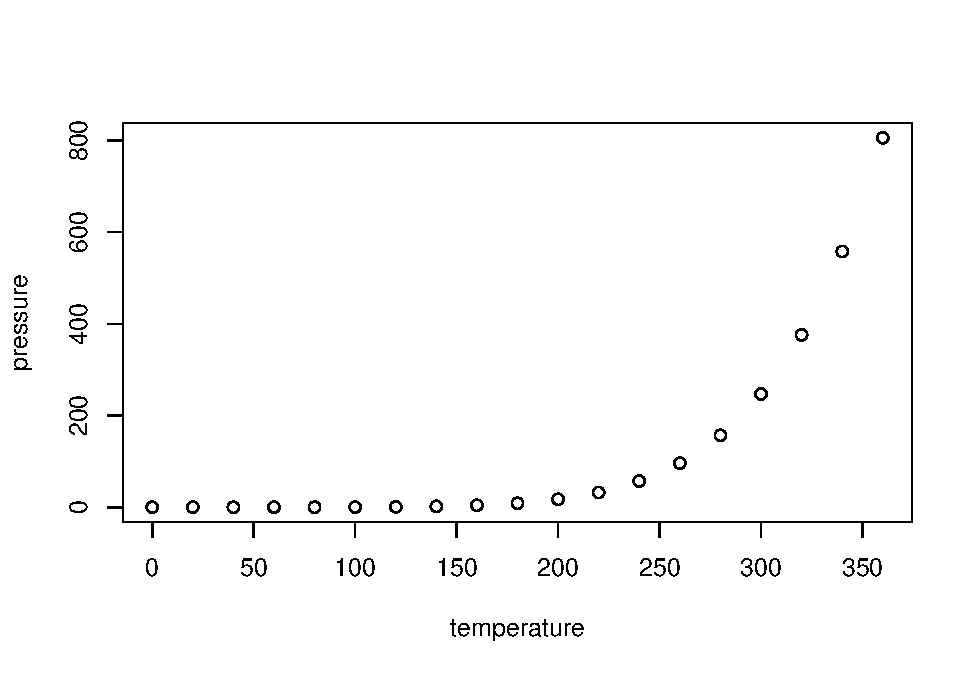
\includegraphics{final_files/figure-latex/unnamed-chunk-2-1} \end{center}

\hypertarget{equazione}{%
\section{Equazione}\label{equazione}}

sempe la stessa, ehehe

\(z = \frac{x_i - \bar{X}}{sd} = \frac{\ensuremath{2\times 10^{-4}}- 124.3367053}{224.6225399 } = -0.5533362\)

\clearpage

\#Risultati di R

Sono risultati di un modello lineare base.

\begin{verbatim}

Call:
lm(formula = pressure ~ temperature, data = data)

Residuals:
    Min      1Q  Median      3Q     Max 
-158.08 -117.06  -32.84   72.30  409.43 

Coefficients:
             Estimate Std. Error t value Pr(>|t|)    
(Intercept) -147.8989    66.5529  -2.222 0.040124 *  
temperature    1.5124     0.3158   4.788 0.000171 ***
---
Signif. codes:  0 '***' 0.001 '**' 0.01 '*' 0.05 '.' 0.1 ' ' 1

Residual standard error: 150.8 on 17 degrees of freedom
Multiple R-squared:  0.5742,    Adjusted R-squared:  0.5492 
F-statistic: 22.93 on 1 and 17 DF,  p-value: 0.000171
\end{verbatim}

Belli vero?

\end{document}
